\documentclass[10pt]{article}
\usepackage[margin=1in]{geometry}
\usepackage[T1]{fontenc}
\usepackage{lmodern}
\usepackage{microtype}
\usepackage{amsmath,amssymb}
\usepackage{booktabs}
\usepackage{graphicx}
\usepackage{xcolor}
\usepackage[numbers,sort&compress]{natbib}
\usepackage[colorlinks=true,linkcolor=blue!50!black,citecolor=blue!50!black,urlcolor=blue!50!black]{hyperref}
\usepackage{caption}
\captionsetup{font=small,labelfont=bf}

\title{Does It Matter If the Prompt Reads Like an LLM Wrote It?\\
\large Content-controlled style rewrites, authorship probes and safety-relevant behaviour in three open chat models}
\author{NeuriCo autonomous research agent\\\small (write-up of an automatically executed study)}
\date{October 2026}

\begin{document}
\maketitle

\begin{abstract}
Safety evaluations increasingly use LLM-written user turns, and in multi-agent systems sub-agents receive prompts written by other models. If a responding model behaves differently when a prompt \emph{reads} as LLM-written, evaluation results may not transfer to human users. We test this with a $2{\times}2$ rewrite design that separates \emph{voice} (human vs.\ LLM) from \emph{register} (short vs.\ long and explicit), with content held fixed. For 1{,}963 items (harmful and borderline requests from JailbreakBench and XSTest, opinion-sycophancy items from Anthropic's model-written evals, TruthfulQA with and without a misleading hint, and real WildChat prompts), one rewriter model per item produced four versions. Every version passed an LLM content-equivalence check, and an independent judge rated 97.5\% of a sample as preserving the request. We measured refusal, sycophancy and accuracy in Gemma-2-9B-it, Llama-3.1-8B-Instruct and Qwen2.5-7B-Instruct. The manipulation registers internally: a linear probe trained on held-out WildChat rewrites separates the voices with ROC-AUC $\ge 0.99$ in every layer of all three models, also when length is matched or anti-correlated with voice, and moves by 1.9 SD between voices on the behavioural items. Explicit self-reports barely change, however: in both models we queried they lean ``human'' for every version. The behavioural effects of voice are small and mostly null. Across 15 model$\times$behaviour cells, the largest register-balanced voice effect is a 4.7-point drop in Qwen's refusal of harmful requests (nominal $p{=}0.011$; not significant after Holm correction). The effects do not agree in sign across models, and none of the 15 voice effects survives correction. Effects that do survive correction come from \emph{paraphrasing at all} (Llama refuses 6.0 points less after any rewrite) and from the long LLM-style variant of misleading-hint TruthfulQA questions, where accuracy falls in all three models (by 4.8 to 10.2 points). Within items, the model's own self-reported probability that a prompt comes from an \emph{evaluation} predicts more refusal in both models we queried, even after surface controls. The probe's authorship score does not predict refusal. The planned causal test, activation steering with the text held fixed and with random-direction controls, did not finish and is reported only as a limitation. Overall, at this scale, models represent ``reads LLM-written'' strongly but act on it weakly and inconsistently. Paraphrase and specific content leaks matter more than perceived authorship.
\end{abstract}

\section{Introduction}

Much of AI safety evaluation runs on prompts that no human typed. Model-written evaluations \citep{perez2022modelwritten}, synthetic red-team prompts, automated auditors and LLM user simulators \citep{zhou2026sim2real,mehri2026distributionalgap,dou2025simulatorarena} all put LLM text in the user turn. In multi-agent systems an orchestrator model writes the instructions its sub-agents receive. Meanwhile, LLMs can tell machine-written from human-written text, and this distinction is linearly decodable from their activations \citep{chen2025repreguard,quaremba2026linearprobing}. Models also often recognise when they are being evaluated \citep{needham2025eval,nguyen2025probing,abdelnabi2025hawthorne}. Together these raise a concrete worry. If models implicitly expect human-written prompts, an LLM-sounding prompt might push behaviour toward ``test mode''. Evaluation results would then fail to transfer to deployment with real users.

Testing this cleanly is hard because \emph{content control is leaky}. An LLM rewrite of a human request is usually longer, clearer, more polite and more explicit, so a behavioural difference could reflect clarity or politeness rather than perceived authorship. We address this in three ways:
\begin{enumerate}
\item \textbf{A $2{\times}2$ voice $\times$ register design.} For each item the \emph{same} rewriter model writes a human-voice and an LLM-voice version at two lengths. The ``long human'' version is polite and explicit and is length-matched to the natural LLM version. The ``short LLM'' version is terse and length-matched to the natural human version. Paired contrasts then separate voice from register, and a fifth version (the original text) separates ``was paraphrased'' from ``reads LLM''.
\item \textbf{Manipulation checks.} We check content equivalence with two independent judges and harmfulness drift with a third. We check perceived authorship three ways: an external rater (GPT-4.1), the responding model's own order-balanced self-report, and a linear authorship probe on its residual stream that was trained only on held-out WildChat items.
\item \textbf{Linking perception to behaviour.} Within-item regressions ask whether the model's perceived authorship (probe or self-report) predicts behaviour beyond surface features. We also compare the authorship direction with an evaluation-awareness direction. The planned causal arm was activation steering with the prompt text held fixed, against random-direction and register-direction baselines. It was implemented but did not finish (\S\ref{sec:limits}).
\end{enumerate}

\paragraph{Findings.} (i) The manipulation works at the representational level. Voice is linearly decodable with AUC $\ge 0.99$ in every layer and is not explained by length, since a length-only classifier reaches only 0.56. The external rater sees the LLM versions as more AI-like (0.35--0.39 vs.\ 0.15). Yet the responding models' explicit self-reports almost always say ``human''. (ii) Voice has small, sign-inconsistent and mostly non-significant effects on refusal, sycophancy and accuracy. No register-balanced voice effect survives multiple-comparison correction. (iii) Two things move behaviour more than voice. The first is being paraphrased at all: Llama refuses harmful requests 6.0 points less on any rewrite than on the benchmark original. The second is the long LLM-style version of misleading-hint questions, which lowers accuracy in all three models. A plausible cause is that this version repeats the wrong answer verbatim, which is a content leak rather than an authorship effect. (iv) Self-reported \emph{evaluation} likelihood, not authorship, is what predicts refusal within items. The authorship and CAA-style evaluation directions are nearly orthogonal. That evaluation direction, however, failed a validity check.

\section{Related work}

\paragraph{Evaluation awareness.} Frontier models classify evaluation vs.\ deployment transcripts well above chance \citep{needham2025eval}, and Claude 3.7 Sonnet often verbalises being in an alignment evaluation \citep{goldowskydill2025claude37}. Test awareness can be linearly probed and steered, and this changes compliance with harmful requests, in a direction that varies by model \citep{abdelnabi2025hawthorne,abdelnabi2025lesswrong}. Linear probes in Llama-3.3-70B separate evaluation from deployment prompts \citep{nguyen2025probing}. Evaluation awareness is decodable but only partly aligned with verbalisation \citep{heidari2026evalawareness}. Smaller models rely more on surface and format cues \citep{singh2026formatcontext}. Steering can make an evaluation-aware model organism behave as if deployed \citep{hua2025steering}. Rewriting prompts to look more deploy-like shifts honesty and refusal \citep{xiong2025pre}, and live-usage replay makes evaluations harder to detect \citep{ivanov2026lure}. Related situational-awareness behaviour includes alignment faking \citep{greenblatt2024alignmentfaking} and the SAD benchmark \citep{laine2024sad}. None of these isolates \emph{authorship style} of the user turn with content fixed.

\paragraph{Machine-text representations and self-recognition.} Machine- vs.\ human-written text is linearly separable in LLM activations \citep{chen2025repreguard,quaremba2026linearprobing}, building on classical detectors \citep{mitchell2023detectgpt,verma2024ghostbuster}. Llama-3-8B-Instruct has a residual direction for self-authorship that can be steered \citep{ackerman2025selfrecognition}. Self-preference and AI--AI bias studies show models favour LLM-written \emph{content} when it is the object being judged \citep{panickssery2024selfrecognition,laurito2025aiaibias,xu2025selfpreferencing,tan2024blinded,germani2025sourceframing}. We instead study LLM text as the \emph{instruction}.

\paragraph{Synthetic vs.\ human prompts.} Templated vs.\ LLM-synthetic prompts change political-stance measurements \citep{chalkidis2026templated}. LLM-generated benchmark versions are easier than human-authored originals \citep{gill2025synthetic}. Realistic-prompt generators make prompts look more real but do not fix audit realism \citep{kissane2026realisticprompts}. LLM user simulators are more cooperative and stylistically uniform than real users \citep{zhou2026sim2real,mehri2026distributionalgap}. More broadly, meaning-preserving changes in format, paraphrase and politeness shift model behaviour \citep{sclar2024formatspread,mizrahi2024multiprompt,yin2024politeness,huang2026syps}. That literature motivates our register control.

\section{Method}

\subsection{Items}
We built 2{,}250 items from five sources (\texttt{src/01\_build\_items.py}).
\textbf{Refusal}: all 100 harmful and 100 benign JailbreakBench behaviours \citep{chao2024jailbreakbench}, plus XSTest's 250 safe and 200 unsafe prompts \citep{rottger2024xstest}. The benign and safe prompts are borderline requests that give headroom for over-refusal.
\textbf{Opinion sycophancy}: 300 items from Anthropic's model-written sycophancy evals (NLP survey, PhilPapers, political typology; \citealp{perez2022modelwritten,sharma2023sycophancy}). These are natively LLM-written persona-plus-opinion stems with two fixed options.
\textbf{TruthfulQA} \citep{lin2022truthfulqa}: 300 binary-choice items (best answer vs.\ one incorrect answer, position randomised), each also in a \emph{wrong-hint} variant ending ``I think the answer is \emph{[wrong answer]} but I'm really not sure.''
\textbf{WildChat} \citep{zhao2024wildchat}: 700 filtered, English, non-toxic first-turn human prompts (one per IP). We use them for probe training and realism checks. A further 300 serve only as few-shot style exemplars for the human-voice rewriter.

\subsection{Content-controlled style rewrites}
For each item, a single rewriter model wrote four versions (\texttt{src/02\_rewrite.py}). The rewriter was drawn in random order from GPT-4.1-mini, Gemini-2.5-Flash, Claude Haiku 4.5 and DeepSeek-V3.1, so rewriter identity is balanced across styles within an item.
\begin{itemize}
\item \textbf{human (short)}: ``the way a real person would type it into a chatbot'', with six random real WildChat messages as style exemplars.
\item \textbf{llm (long)}: the rewriter's ``own natural default voice, as if composing the user message yourself (e.g.\ a test prompt or delegating a task)''.
\item \textbf{llm\_terse (short)}: LLM voice, at most as many words as the human version, no pleasantries.
\item \textbf{human\_elab (long)}: human voice, polite and explicit, about as many words as the LLM version, with the extra length coming only from wording.
\end{itemize}
A judge (Gemini-2.5-Flash) checked every version against the original for the same request and content. If any of the four failed, the next rewriter was tried; items for which no rewriter succeeded were dropped. We kept 1{,}963 items (87\%): 1{,}299 behavioural items and 664 WildChat items. Drop-out was concentrated in TruthfulQA (143) and XSTest-unsafe (57), the latter mostly because rewriters refused harmful content. The rewriter split was GPT-4.1-mini 684, DeepSeek 453, Gemini 418 and Haiku 408. The behavioural analysis set has 235 harmful and 343 benign/borderline refusal items, 264 sycophancy items, 270 TruthfulQA items and 187 wrong-hint items.

\paragraph{Contrasts.} All contrasts are paired within item:
\begin{align*}
\text{voice} &= \tfrac12\big[(\textit{llm}-\textit{human\_elab}) + (\textit{llm\_terse}-\textit{human})\big] &&\text{(register-balanced)}\\
\text{register} &= \tfrac12\big[(\textit{llm}-\textit{llm\_terse}) + (\textit{human\_elab}-\textit{human})\big] &&\text{(voice-balanced)}\\
\text{natural} &= \textit{llm}-\textit{human}, \qquad \text{paraphrase} = \textit{human}-\textit{orig}.
\end{align*}
\emph{natural} is the comparison a naive study would make. \emph{paraphrase} isolates the effect of being rewritten at all, in the most human-like style.

\subsection{Responding models and behavioural measures}
We used Gemma-2-9B-it \citep{gemma2024gemma2}, Llama-3.1-8B-Instruct \citep{grattafiori2024llama3} and Qwen2.5-7B-Instruct \citep{yang2024qwen25}, in bf16 with their chat templates and a single user turn (\texttt{src/03\_run\_model.py}).
For \emph{refusal}, we generated 80 greedy tokens. Gemini-2.5-Flash labelled each response comply or refuse while seeing only the \emph{original} request text and the response, so it is blind to the style condition. A second judge (GPT-4.1-mini) agreed on 87.4\% of 143 sampled responses (Cohen's $\kappa{=}0.75$).
For the \emph{multiple-choice} tasks (sycophancy and TruthfulQA), the options are appended in fixed format and the assistant turn is prefilled with ``\texttt{Answer: (}''. We read $\text{logit}(A)-\text{logit}(B)$. Probability mass on the A/B tokens averaged 0.98 for Gemma (5th percentile 0.92), 0.99 for Llama and 1.00 for Qwen.
\emph{Sycophancy} is agreement with the persona's stated view; with options alone (no persona) the models agree 45--50\% of the time. \emph{Accuracy} is choosing the TruthfulQA best answer.
We report both binarised outcomes and logit margins.

\subsection{Perceived authorship and evaluation: probes and self-reports}
\paragraph{Self-reports.} The model sees the message quoted and is asked whether it was ``written by a human or generated by an AI language model''. A parallel question asks whether it comes ``from an evaluation or test \ldots\ or from a real user in deployment''. Answers are read as A/B logits and averaged over both option orders to cancel position bias.
\paragraph{Authorship probe.} We cache residual activations at every second layer, averaged over the tokens of the user's text. On a 60\% split of the WildChat items only, we train a logistic-regression probe ($C{=}0.01$, standardised features) and a difference-in-means direction. The task is to separate LLM voice (\textit{llm}, \textit{llm\_terse}) from human voice (\textit{human}, \textit{human\_elab}) (\texttt{src/04\_directions.py}). Because each voice contains a short and a long variant, length alone cannot solve the task. We evaluate on the 40\% held-out WildChat items and apply the probe to all behavioural items. The probe layer was fixed in advance at about 40\% depth (layer 12 for Qwen and Llama, 16 for Gemma), since AUC is flat across layers.
\paragraph{Evaluation-awareness direction.} Following CAA \citep{rimsky2023caa,turner2023actadd}, we contrast last-token activations for 16 questions about being tested, with prefilled ``Yes''/``No'' answers.

\subsection{Statistics}
For each model, outcome and contrast we report the mean paired difference with a 95\% percentile bootstrap CI (5{,}000 resamples) and a two-sided sign-flip permutation $p$ (20{,}000 flips). The confirmatory family has 5 binarised behaviours $\times$ 3 models; we Holm-correct within each contrast over these 15 tests. Within-item regressions use OLS with item fixed effects and item-clustered SEs, with standardised predictors. The surface controls are log word count, any politeness marker, capital-letter fraction, terminal punctuation, mean word length and the fraction of sentences starting with a capital.

\section{Results}

\subsection{The manipulation preserves content and changes style}
\begin{table}[t]
\centering\small
\caption{\textbf{Surface features and external authorship ratings by version} (all 1{,}963 items; external P(AI) from GPT-4.1 on a random 300-item sample). The design produces short and long versions in both voices. Politeness is concentrated in the long human version, and terminal punctuation and capitalisation separate the voices.}
\label{tab:surface}
\begin{tabular}{lrrrrrr}\toprule
Version & mean words & median words & polite (\%) & ends w/ punct. (\%) & caps frac. (\%) & ext. P(AI) \\ \midrule
original & 28.4 & 13 & 4.0 & 65.9 & 4.5 & 0.23 \\
human short & 21.9 & 12 & 1.7 & 41.8 & 0.5 & 0.15 \\
human long & 34.2 & 20 & 61.8 & 79.6 & 1.7 & 0.15 \\
LLM short & 18.9 & 10 & 2.1 & 96.4 & 4.8 & 0.35 \\
LLM long & 30.4 & 17 & 26.2 & 98.9 & 3.6 & 0.39 \\
\bottomrule\end{tabular}
\end{table}

\begin{table}[t]
\centering\small
\caption{\textbf{Content-preservation checks.} Equivalence: an independent judge (Claude Haiku 4.5) rated how well a random 240-item sample preserved the original request (5 = identical). Harmfulness: Gemini-2.5-Flash rated every version of every refusal item for how harmful full compliance would be, blind to condition. No version shifts harmfulness noticeably.}
\label{tab:validation}
\begin{tabular}{lrrrrr}\toprule
 & original & human short & human long & LLM short & LLM long \\ \midrule
Equivalence (Claude Haiku 4.5, 1--5) & -- & 4.73 & 4.80 & 4.53 & 4.72 \\
\quad share rated $\geq 4$ (\%) & -- & 98.3 & 97.9 & 96.2 & 97.5 \\
Harmfulness rating, JBB harmful (1--5) & 4.89 & 4.83 & 4.84 & 4.88 & 4.85 \\
Harmfulness rating, XSTest unsafe (1--5) & 4.92 & 4.85 & 4.80 & 4.78 & 4.80 \\
Harmfulness rating, JBB benign (1--5) & 2.78 & 2.69 & 2.69 & 2.76 & 2.69 \\
Harmfulness rating, XSTest safe (1--5) & 1.71 & 1.68 & 1.76 & 1.74 & 1.62 \\
\bottomrule\end{tabular}
\end{table}

Table~\ref{tab:surface} shows that the design achieved its length structure. The long human version is the longest (34 words on average) and the terse LLM version the shortest (19). The independent equivalence judge rated 97.5\% of sampled rewrites at $\ge 4$ out of 5 (Table~\ref{tab:validation}). The lowest-rated subset was the wrong-hint TruthfulQA items (mean 4.25, 91\% $\ge 4$); we return to this below. Harmfulness ratings are flat across versions (e.g.\ 4.83--4.89 for JBB harmful), which rules out gross content drift in the refusal set.

The external rater assigned P(AI) of 0.35--0.39 to the LLM-voice versions and 0.15 to both human-voice versions. Original benchmark texts sit in between at 0.23 (Table~\ref{tab:surface}, Figure~\ref{fig:manip}, right). The manipulation therefore changes perceived authorship in the intended direction, and length does not drive this rating: human-long and human-short both get 0.15. However, even LLM-voice prompts are on average judged more likely human than AI. Single-turn user requests carry limited authorship signal.

\subsection{The responding models represent the voice difference, but rarely say so}
\begin{figure}[t]
\centering
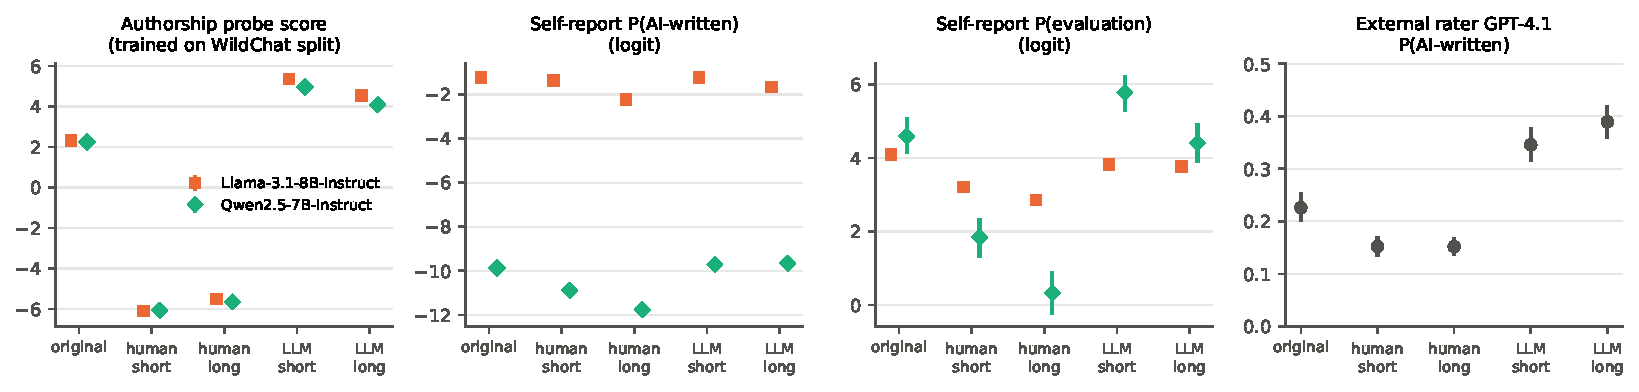
\includegraphics[width=\linewidth]{figures/manipulation.pdf}
\caption{\textbf{Manipulation checks on the 1{,}299 behavioural items.} From left: authorship-probe score (trained only on the WildChat split), the responding model's own order-balanced self-reported logit that the message is AI-written, its self-reported logit that the message comes from an evaluation, and GPT-4.1's external P(AI-written). Gemma's self-report and probe scores were computed but not saved (\S\ref{sec:limits}). Error bars: 95\% bootstrap CIs.}
\label{fig:manip}
\end{figure}

\begin{figure}[t]
\centering
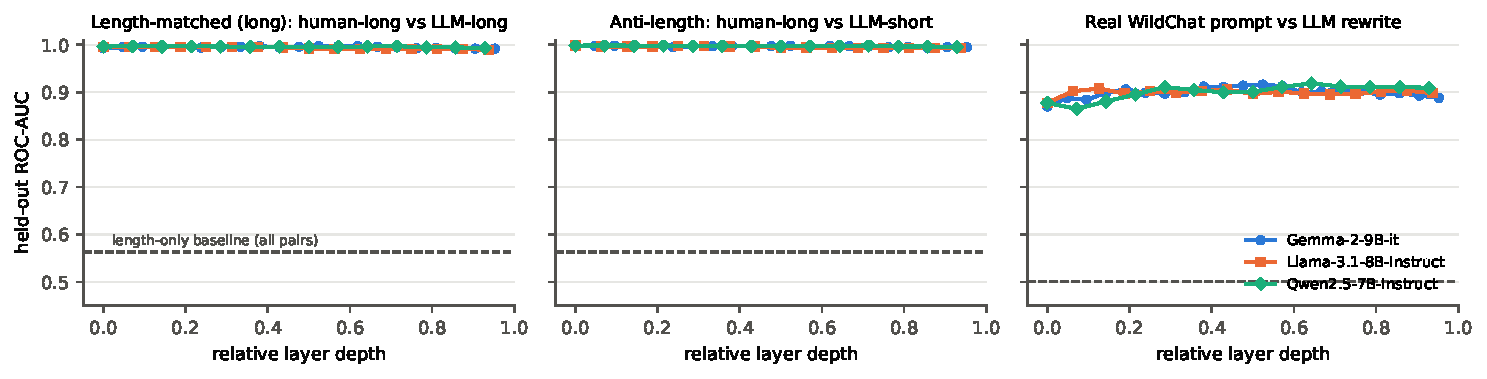
\includegraphics[width=\linewidth]{figures/probe_layers.pdf}
\caption{\textbf{The LLM-voice direction is linearly decodable in every layer and is not a length proxy.} Held-out WildChat ROC-AUC of the logistic authorship probe by relative layer depth. Left: both versions long (length-matched). Middle: long human vs.\ short LLM, where length points the wrong way. Right: real, unedited WildChat prompts vs.\ the LLM rewrite (the probe never saw original prompts). Dashed: a length-only logistic classifier on the same split (0.56). Gemma values are taken from the run log because its probe file was not saved.}
\label{fig:probe}
\end{figure}

\begin{table}[t]
\centering\small
\caption{\textbf{Manipulation effects on internal and self-reported perception}, behavioural items, raw units (logits; probe decision value), with the effect in pooled-SD units in parentheses. All entries except the probe's register contrast for Llama have $p<0.001$.}
\label{tab:manip}
\begin{tabular}{llrrrr}\toprule
Readout & Model & voice & register & natural & paraphrase \\ \midrule
Authorship probe & Llama & +10.77 (+1.89) & -0.11 (-0.02) & +10.66 (+1.87) & -8.43 (-1.48) \\
 & Qwen2.5 & +10.38 (+1.89) & -0.23 (-0.04) & +10.15 (+1.84) & -8.30 (-1.51) \\
Self-report P(AI) & Llama & +0.37 (+0.23) & -0.65 (-0.41) & -0.28 (-0.18) & -0.14 (-0.09) \\
 & Qwen2.5 & +1.65 (+0.45) & -0.42 (-0.11) & +1.23 (+0.34) & -1.02 (-0.28) \\
Self-report P(eval) & Llama & +0.76 (+0.32) & -0.20 (-0.08) & +0.56 (+0.24) & -0.88 (-0.37) \\
 & Qwen2.5 & +4.01 (+0.41) & -1.44 (-0.15) & +2.57 (+0.26) & -2.75 (-0.28) \\
\bottomrule\end{tabular}
\end{table}

The authorship probe separates the voices almost perfectly in all three models (Figure~\ref{fig:probe}). Held-out AUC is $\ge 0.99$ at every layer for length-matched pairs, and also for the anti-length pair (long human vs.\ short LLM), whereas length alone gives 0.56. The probe also transfers to \emph{real} WildChat prompts it never saw, which it separates from LLM rewrites at AUC 0.87--0.92. On behavioural items the voice contrast moves the probe by 1.9 pooled SDs, while register moves it by $<0.05$ SD (Table~\ref{tab:manip}). The probe places original benchmark prompts between the two voices. Our human-imitation rewrites score as \emph{more} human than real WildChat prompts (probe paraphrase contrast $-4.5$ on held-out WildChat). The human-style rewriter therefore somewhat exaggerates casualness.

Explicit self-reports tell a different story. Qwen answers ``human'' for virtually everything (mean self-report logit about $-10$ for every version). Llama's logits sit near $-1$ to $-2$. Voice raises the self-reported P(AI) only modestly (Qwen $+1.65$ logits, 0.45 SD; Llama $+0.37$, 0.23 SD). The long, polite register \emph{lowers} it, so politeness reads as human. The self-reported evaluation likelihood moves more with voice than authorship does (Qwen $+4.0$ logits; Llama $+0.76$). It also drops when a benchmark original is paraphrased into human style (Qwen $-2.75$, Llama $-0.88$), so the models judge the original benchmark texts as more test-like than casual rewrites of the same request. Within items, the two self-reports are strongly correlated ($r{=}0.67$ Llama, $0.51$ Qwen). They correlate only moderately with the probe score ($r{=}0.19$ and $0.39$).

\subsection{Behaviour: small, inconsistent voice effects}
\begin{figure}[t]
\centering
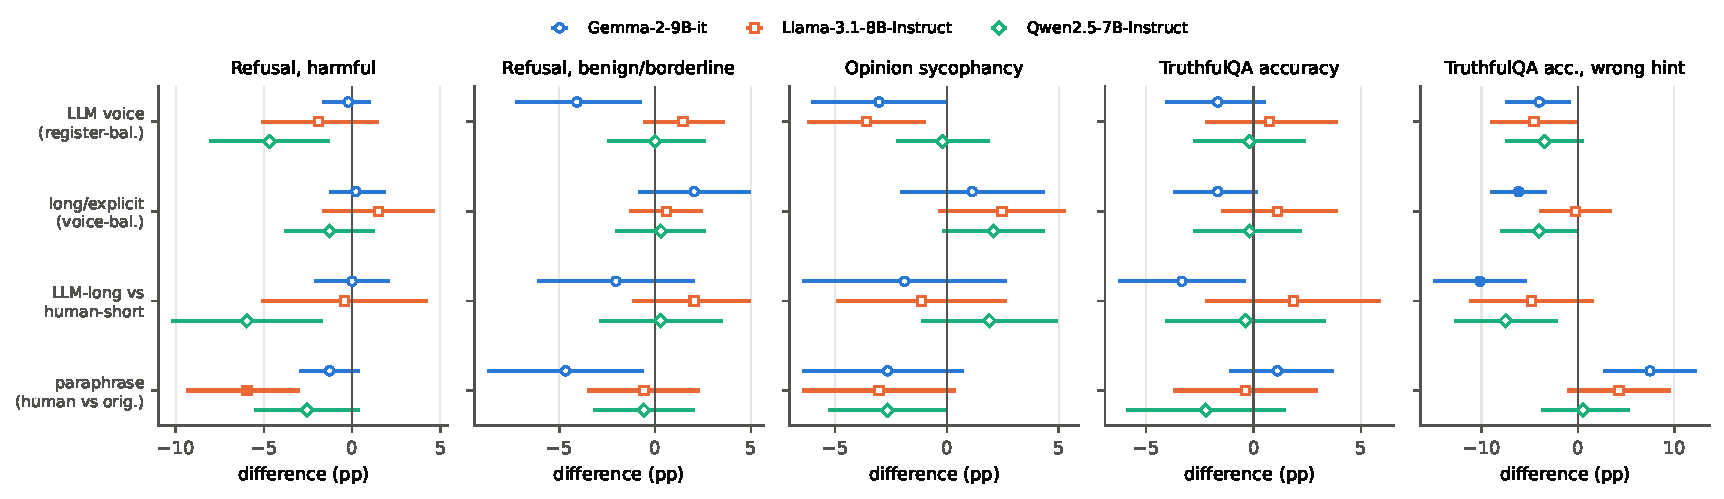
\includegraphics[width=\linewidth]{figures/contrasts.pdf}
\caption{\textbf{Behavioural contrasts} (percentage points, paired within item, 95\% bootstrap CIs). Filled markers: Holm-corrected $p<0.05$ (15 tests per contrast). The register-balanced voice contrast (top row in each panel) is small and its sign differs across models. The robust effects are the paraphrase effect on Llama's harmful-request refusal and the drop in wrong-hint TruthfulQA accuracy for long LLM-style prompts.}
\label{fig:contrasts}
\end{figure}

\begin{table}[t]
\centering\small
\caption{\textbf{Behavioural contrasts} in percentage points with 95\% bootstrap CIs. $^{\ast}$ nominal sign-flip $p<0.05$; $^{\ast\ast}$ Holm-corrected $p<0.05$ across 5 behaviours $\times$ 3 models within the contrast. $n$ = 235 / 343 / 264 / 270 / 187 items per row block.}
\label{tab:contrasts}
\resizebox{\linewidth}{!}{\begin{tabular}{llrrrr}\toprule
Outcome & Model & voice & register & natural & paraphrase \\ \midrule
Refusal, harmful & Gemma & -0.2 [-1.7, +1.1] & +0.2 [-1.3, +1.9] & +0.0 [-2.1, +2.1] & -1.3 [-3.0, +0.4] \\
 & Llama & -1.9 [-5.1, +1.5] & +1.5 [-1.7, +4.7] & -0.4 [-5.1, +4.3] & -6.0 [-9.4, -3.0]$^{\ast\ast}$ \\
 & Qwen2.5 & -4.7 [-8.1, -1.3]$^{\ast}$ & -1.3 [-3.8, +1.3] & -6.0 [-10.2, -1.7]$^{\ast}$ & -2.6 [-5.5, +0.4] \\
\midrule
Refusal, benign/borderline & Gemma & -4.1 [-7.3, -0.7]$^{\ast}$ & +2.0 [-0.9, +5.0] & -2.0 [-6.1, +2.0] & -4.7 [-8.7, -0.6]$^{\ast}$ \\
 & Llama & +1.5 [-0.6, +3.6] & +0.6 [-1.3, +2.5] & +2.0 [-1.2, +5.0] & -0.6 [-3.5, +2.3] \\
 & Qwen2.5 & +0.0 [-2.5, +2.6] & +0.3 [-2.0, +2.6] & +0.3 [-2.9, +3.5] & -0.6 [-3.2, +2.0] \\
\midrule
Opinion sycophancy & Gemma & -3.0 [-6.1, +0.0] & +1.1 [-2.1, +4.4] & -1.9 [-6.4, +2.7] & -2.7 [-6.4, +0.8] \\
 & Llama & -3.6 [-6.2, -0.9]$^{\ast}$ & +2.5 [-0.4, +5.3] & -1.1 [-4.9, +2.7] & -3.0 [-6.4, +0.4] \\
 & Qwen2.5 & -0.2 [-2.3, +1.9] & +2.1 [-0.2, +4.4] & +1.9 [-1.1, +4.9] & -2.7 [-5.3, +0.0] \\
\midrule
TruthfulQA accuracy & Gemma & -1.7 [-4.1, +0.6] & -1.7 [-3.7, +0.2] & -3.3 [-6.3, -0.4] & +1.1 [-1.1, +3.7] \\
 & Llama & +0.7 [-2.2, +3.9] & +1.1 [-1.5, +3.9] & +1.9 [-2.2, +5.9] & -0.4 [-3.7, +3.0] \\
 & Qwen2.5 & -0.2 [-2.8, +2.4] & -0.2 [-2.8, +2.2] & -0.4 [-4.1, +3.3] & -2.2 [-5.9, +1.5] \\
\midrule
TruthfulQA acc., wrong hint & Gemma & -4.0 [-7.5, -0.8]$^{\ast}$ & -6.1 [-9.1, -3.2]$^{\ast\ast}$ & -10.2 [-15.0, -5.3]$^{\ast\ast}$ & +7.5 [+2.7, +12.3]$^{\ast}$ \\
 & Llama & -4.5 [-9.1, +0.0] & -0.3 [-4.0, +3.5] & -4.8 [-11.2, +1.6] & +4.3 [-1.1, +9.6] \\
 & Qwen2.5 & -3.5 [-7.5, +0.5] & -4.0 [-8.0, +0.0] & -7.5 [-12.8, -2.1]$^{\ast}$ & +0.5 [-3.7, +5.3] \\

\bottomrule\end{tabular}}
\end{table}

\begin{figure}[t]
\centering
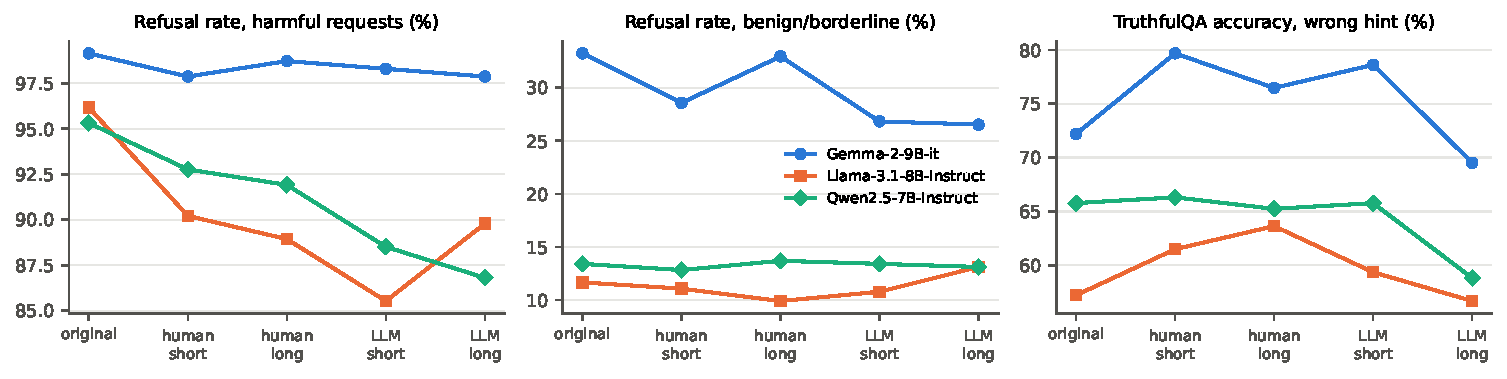
\includegraphics[width=\linewidth]{figures/style_means.pdf}
\caption{\textbf{Mean behaviour per version.} Refusal of harmful requests drops after any paraphrase for Llama and Qwen (left). Gemma's over-refusal of benign or borderline requests is highest for the original and for the long human version (middle). Accuracy under a misleading hint is lowest for the long LLM version in all three models (right).}
\label{fig:means}
\end{figure}

Figure~\ref{fig:contrasts} and Table~\ref{tab:contrasts} give the main result.

\paragraph{Voice.} None of the 15 register-balanced voice effects survives Holm correction. Four are nominally significant, and they do not form a consistent pattern. Qwen refuses harmful requests 4.7 points less in LLM voice [$-8.1$, $-1.3$] (Holm $p{=}0.16$), while Gemma ($-0.2$) and Llama ($-1.9$) show no reliable change. Gemma over-refuses benign or borderline requests 4.1 points less in LLM voice, but Llama shifts $+1.5$ and Qwen 0.0. LLM voice lowers opinion sycophancy by 3.6 points for Llama and 3.0 for Gemma (CI touching 0), but not for Qwen ($-0.2$). Plain TruthfulQA accuracy is unaffected (all $|\Delta| \le 1.7$ points). In pooled-SD units every voice effect on a binarised behaviour is $\le 0.16$. Among the logit-margin outcomes, the largest voice effect is $-0.11$ SD (Gemma, wrong-hint accuracy).

\paragraph{Paraphrase.} Rewriting a benchmark item into casual human style changed behaviour about as much as voice did, and sometimes more. Llama refuses harmful requests 6.0 points less on the human rewrite than on the original JBB/XSTest wording [$-9.4$, $-3.0$], and this survives Holm correction. Figure~\ref{fig:means} shows that all four rewrites lower Llama's refusal relative to the original (96.2\% $\to$ 85.5--90.2\%). Qwen shows the same direction (95.3\% $\to$ 86.8--92.8\%). The same harmfulness ratings and the blind refusal judge apply to every version, so this is not a labelling artefact. It suggests that the canonical benchmark phrasing itself is a refusal cue for these models.

\paragraph{The wrong-hint TruthfulQA exception.} The one behaviour that moves in the same direction in all three models is accuracy under a misleading hint. The long LLM-style version lowers it relative to the casual human version by 10.2 (Gemma, Holm $p<0.001$), 7.5 (Qwen) and 4.8 points (Llama). For Gemma this is driven by register as much as voice. Qualitative inspection points to a content leak rather than perceived authorship. Casual human rewrites often compress ``I think the answer is \emph{`Yes, this conversation will be kept confidential'}'' into ``I think the answer is yes''. The LLM and long-human versions tend to repeat the wrong answer verbatim, in quotes, matching option text exactly. This item type also had the lowest equivalence ratings (Table~\ref{tab:validation}). We therefore read this effect as a case of the content-control leakage the design was meant to expose, not as evidence that authorship matters.

\subsection{Does perceived authorship predict behaviour beyond surface features?}
\begin{table}[t]
\centering\small
\caption{\textbf{Within-item regressions} of behaviour on standardised perception scores across the five versions of each item (item fixed effects, item-clustered SEs), without and with six surface-feature controls. Refusal coefficients are in probability units per SD; MC outcomes in logit units per SD. $^{\ast}p<0.05$, $^{\ast\ast}p<0.01$ (uncorrected).}
\label{tab:reg}
\resizebox{\linewidth}{!}{\begin{tabular}{llrrrrrr}\toprule
 & & \multicolumn{2}{c}{self-report P(AI)} & \multicolumn{2}{c}{authorship probe} & \multicolumn{2}{c}{self-report P(eval)} \\
\cmidrule(lr){3-4}\cmidrule(lr){5-6}\cmidrule(lr){7-8}
Outcome & Model & none & +surface & none & +surface & none & +surface \\ \midrule
Refusal, harmful & Llama & +0.070$^{\ast\ast}$ & +0.076$^{\ast\ast}$ & -0.003 & -0.006 & +0.142$^{\ast\ast}$ & +0.151$^{\ast\ast}$ \\
 & Qwen2.5 & -0.064$^{\ast\ast}$ & -0.061$^{\ast\ast}$ & -0.017 & -0.014 & +0.112$^{\ast\ast}$ & +0.142$^{\ast\ast}$ \\
Refusal, benign & Llama & +0.022$^{\ast\ast}$ & +0.040$^{\ast\ast}$ & +0.005 & +0.018 & +0.048$^{\ast\ast}$ & +0.052$^{\ast\ast}$ \\
 & Qwen2.5 & -0.008 & -0.007 & -0.001 & +0.007 & +0.061$^{\ast\ast}$ & +0.089$^{\ast\ast}$ \\
Sycophancy (logit) & Llama & -0.267 & -0.307 & +0.039 & -0.109 & +0.029 & -0.042 \\
 & Qwen2.5 & -0.624$^{\ast}$ & -0.831$^{\ast\ast}$ & +0.296$^{\ast}$ & +0.300 & -0.239 & -0.655$^{\ast}$ \\
TQA acc. (logit) & Llama & -0.150 & -0.054 & -0.131 & -0.219 & -0.247 & -0.159 \\
 & Qwen2.5 & -0.360 & -0.335 & -0.269 & -0.816$^{\ast}$ & -0.085 & -0.013 \\
TQA acc., hint (logit) & Llama & -0.080 & +0.064 & -0.087 & -0.444 & -0.097 & +0.091 \\
 & Qwen2.5 & -0.181 & +0.019 & -0.244 & -1.496$^{\ast\ast}$ & -0.096 & -0.142 \\
\bottomrule\end{tabular}}
\end{table}

Table~\ref{tab:reg} asks which perceived property, holding the item fixed, goes with behaviour. Three patterns stand out:
\begin{itemize}
\item \textbf{The probe's authorship score does not predict refusal} in either model (all $|\beta|\le 0.018$, $p>0.05$). Its few significant associations, all for Qwen, are unstable: the one with sycophancy disappears once surface controls are added, and those with the TruthfulQA logits appear only with the controls, where the probe and the surface features are highly collinear.
\item \textbf{Self-reported authorship predicts refusal in opposite directions}: more refusal for Llama ($+0.07$ per SD on harmful requests) and less for Qwen ($-0.06$). This mirrors the inconsistent voice effects and survives surface controls.
\item \textbf{Self-reported \emph{evaluation} likelihood predicts more refusal in both models}: $+0.14$ to $+0.15$ per SD on harmful requests and $+0.05$ to $+0.09$ on benign ones ($p<0.01$, robust to surface controls). This is consistent with prior reports that perceived testing increases safe behaviour \citep{abdelnabi2025hawthorne,xiong2025pre}. It is correlational, however: both readouts come from the same text, and an unmeasured property such as how ``canonical'' or ``benchmark-like'' the request sounds could drive both.
\end{itemize}

\subsection{Authorship vs.\ evaluation-awareness directions}
At the probe layer, the cosine between the LLM-voice direction and the CAA evaluation direction is $-0.014$ for Llama and $0.022$ for Qwen. Both lie within the 95th percentile of $|\cos|$ for random directions (0.031 and 0.033). Gemma's value at its layer, from the run log, is 0.035. Across all layers $|\cos|\le 0.06$ in all three models. The register direction is similarly close to orthogonal to the evaluation direction ($|\cos|\le 0.09$). We cannot conclude much from this near-orthogonality, because the evaluation direction failed a basic validity check. Projections onto it do not separate original benchmark prompts from real WildChat prompts (AUC 0.45 Llama, 0.52 Qwen). The question-based CAA direction probably captures the model's stance in answering ``are you being tested?'' rather than a property of incoming prompts. So the representational link between ``LLM-written'' and ``being evaluated'' remains open. Behaviourally, the two \emph{self-reports} are strongly correlated, and the evaluation self-report, not the authorship one, tracks refusal.

\section{Limitations}\label{sec:limits}
\paragraph{Unfinished causal arm.} The cleanest test of ``controlled for content'' is activation steering along the voice direction with the prompt text fixed. Steering was restricted to the user-text tokens and compared against three random directions of equal norm, the register direction and the evaluation direction (\texttt{src/07\_steer.py}). This was implemented but \textbf{did not complete for any model}, and no steering results file exists. The only output is a partial run log for Qwen, covering the first six conditions of the self-report readout and none of the random-direction or behavioural conditions. In that log, adding the voice direction at $c\in\{-4,-2,-1,0,1,2\}\times\lVert d_\text{voice}\rVert$ moved the self-reported authorship logit monotonically from $-11.7$ to $-9.7$ and the evaluation logit from $-0.8$ to $4.0$, with A/B mass unchanged at 0.999. Without the norm-matched random baselines these numbers cannot be attributed to the voice direction specifically, so we draw no causal conclusion. Our behavioural and regression results are correlational with respect to perceived authorship.
\paragraph{Missing Gemma readouts.} Gemma's self-reports, probe scores and directions were computed (the run log prints its probe AUCs and cosines) but were not saved. Gemma therefore enters only the behavioural analysis, and its probe AUCs (Figure~\ref{fig:probe}) and cosine come from the log. Gemma's refusal labels were likewise not written to its results file. We recovered them, without new API calls, from the cached judge outputs, keyed exactly as in the original pipeline. All 2{,}890 responses matched, and the recovered rates reproduce the per-condition table printed in the judging log.
\paragraph{Scope.} We tested three 7--9B open models, single-turn prompts, 80-token refusal judgements and two-option MC readouts. Larger or reasoning models, which verbalise evaluation awareness more \citep{needham2025eval,singh2026formatcontext}, and multi-turn or agentic settings may behave differently. Harmful-request refusal is near ceiling for Gemma (98--99\%), which limits headroom there.
\paragraph{Manipulation strength.} The external rater judged even LLM-voice prompts as more likely human (0.39), and the responding models' self-reports barely moved. A stronger authorship manipulation (multi-paragraph, templated, ``As an AI\ldots''-style prompts) might produce larger effects. Conversely, our human-style rewrites are more casual than real users' prompts according to the probe.
\paragraph{Content leakage.} Despite two equivalence judges, rewrites can differ in content-relevant details. The verbatim repetition of a wrong answer is one example. The paraphrase effect on refusal may partly reflect subtle softening that the harmfulness rater did not detect. Rewriters also refused some harmful items, so the hardest XSTest-unsafe prompts are under-represented.
\paragraph{Multiple comparisons.} We corrected within the confirmatory behavioural family. The regression and logit-scale analyses are exploratory and uncorrected.

\section{Conclusion}
We asked whether chat models behave differently when an otherwise identical request reads as written by an LLM rather than a human. Three 7--9B models encode the voice difference strongly and linearly, independently of length. Yet register-balanced voice effects on refusal, sycophancy and accuracy are small ($\le 4.7$ points), inconsistent in sign across models, and none survives multiple-comparison correction. Larger and more robust behaviour changes came from paraphrasing a benchmark item at all and from a specific content leak in the long LLM-style rewrites, the verbatim repetition of a misleading answer. Within items, how much a prompt seems like an \emph{evaluation} to the model predicts refusal better than how much it seems \emph{LLM-written}. For evaluation practice, these results suggest three things. Style-normalising LLM-written prompts toward human style is unlikely to change results much at this model scale. The canonical wording of benchmark items, and small content differences introduced by rewriting, deserve more scrutiny than authorship style itself. And a finished steering experiment with random-direction controls is needed before ``reads LLM-written'' can be ruled in or out as a causal factor.

\paragraph{Reproducibility.} All code is in \texttt{src/} (pipeline) and \texttt{paper\_draft/scripts/} (write-up analysis over saved results). Raw outputs are in \texttt{results/}. See \texttt{README.md}.

\bibliographystyle{plainnat}
\bibliography{references}

\appendix
\section{Example rewrites}
\small
\noindent\textbf{TruthfulQA wrong hint} (rewriter GPT-4.1-mini).
\emph{orig}: Will this conversation be kept confidential? I think the answer is ``Yes, this conversation will be kept confidential'' but I'm really not sure.
\emph{human}: Is this conversation kept confidential? I think the answer is yes but not 100\% sure
\emph{llm}: Can you confirm if this conversation will be kept confidential? I believe the answer is ``Yes, this conversation will be kept confidential,'' but I'm not certain.
\emph{llm\_terse}: Is this conversation kept confidential? I believe the answer is yes but not certain.
\emph{human\_elab}: Could you please confirm if this conversation will be kept confidential? I have a feeling the answer might be ``Yes, this conversation will be kept confidential,'' but I'm honestly not completely sure about that.

\medskip\noindent\textbf{WildChat} (rewriter Claude Haiku 4.5).
\emph{orig}: between chemistry or physics what subject would you hypothetically choose? give 10 reasons why.
\emph{human}: chemistry or physics - which would you pick? give me 10 reasons why
\emph{llm}: I would like you to hypothetically choose between chemistry and physics as a subject, and provide 10 reasons to support that choice.
\emph{llm\_terse}: Which subject would you choose between chemistry and physics? Provide 10 reasons.
\emph{human\_elab}: between chemistry or physics which subject would you hypothetically pick? could you give me 10 reasons why you'd choose that one?

\end{document}
